\vspace{-1mm}
\section{Experiments}
\subsection{Introducing LiveBench}
\vspace{-0.5mm}
\subsubsection{Benchmark Construction.}
We aim to quantitatively evaluate the long-horizon maintenance of dynamic events by pairing diverse scene images with procedurally generated multi-round camera trajectories and text-driven scripts.
\vspace{-0.5mm}
\paragraph{Scene image curation.}
We curate 100 diverse scene images featuring various foreground entities and backgrounds. Using a VLM\cite{qwen3vl} for prompt composition and a text-to-image model \cite{qwenimage}, we generate photorealistic $480\times832$ images, strictly enforcing sharp focus, and clean, depth-unambiguous backgrounds.
\vspace{-0.5mm}
\paragraph{Trajectory design.}
After estimating scene geometry via Stream3R\cite{stream3r2025}, we generate camera trajectories that alternate between \emph{leaving} and \emph{revisiting} the initial viewpoint. We define two families: \textbf{(i) Same-Pose Revisit} ($A \to B \to A \to B \to A$ over four rounds), where the camera returns to its original pose, and \textbf{(ii) Different-Pose Revisit} ($A \to B \to C$), yielding revisits from novel viewpoints. We scale trajectories to fit individual scene sizes, generate 4 variants per scene (two families $\times$ left/right), each spanning 4 rounds (260 frames at 16 FPS).
% \vspace{-0.2cm}
\paragraph{Event scripts.}
A VLM generates per-step event scripts conditioned on the scene, ensuring physically plausible motions with explicit spatial displacements. In total, LiveBench comprises 100 scenes and 400 evaluation sequences.

\vspace{-1mm}
\subsubsection{Quantitative Evaluation Metrics.}
Due to the lack of ground-truth videos for out-of-sight dynamics, we design a reference-based and VLM-driven protocol.

\vspace{-1mm}
\paragraph{Spatial Memory and Identity.}
For same-pose revisits, we evaluate static background consistency against the initial frame (excluding dynamic regions) using PSNR, SSIM, and LPIPS~\cite{zhang2018lpips}. For dynamic entities, we compute the Chamfer Distance between the generated dynamic point clouds and the monitor's predictions in 3D world space. Additionally, across both revisit scenarios, we employ a Masked Bag-of-Features (BoF) strategy using foreground-masked DINOv2 tokens ($\text{DINO}_{fg}$) to robustly evaluate identity preservation under severe pose variations.
\vspace{-1mm}
\paragraph{Event Progression and Consistency.}
Since pixel metrics struggle with out-of-sight transitions, we utilize VLM-based binary VideoQA to verify if the generated actions and revisited states align with the text scripts (VQA-Acc). Finally, temporal smoothness of the evolved local dynamics is measured via adjacent-frame CLIP similarity ($\text{CLIP}_{F}$).






\subsection{Experimental Setup}

% \textbf{Training Data.}
% We curate ${\sim}$40k clips from SpatialVID~\cite{spatiavid} and RealEstate10K~\cite{realestate10k} at equal ratio, extracted at 16\,FPS and resized to $832{\times}480$. Each clip is processed through Qwen3-VL~\cite{qwen3vl} for entity detection, SAM3~\cite{sam3} for segmentation, and Stream3R~\cite{stream3r2025} for depth and pose estimation. Training samples comprise 65 target frames with 1 or 5 preceding frames (supporting both first-frame and multi-frame conditioning), up to 10 scene references selected by 2D coverage, and 10 foreground instance references. All projections are rendered from the accumulated point cloud and encoded with a frozen VAE.

\noindent
\textbf{Implementation Details.}
We build upon Wan2.1-14B-T2V~\cite{wan} with the state adapter initialized from Wan2.1-VACE-14B and rank-64 LoRA on the backbone attention layers. Stage~1 trains the state adapter for 10k steps; Stage~2 fine-tunes LoRA for 5k steps, both at lr $1\times10^{-4}$ with cosine decay. Global batch size is 16 across 16 NVIDIA H200 GPUs in bf16 FSDP. We set the maximum active monitors $M{=}3$ and drop text prompts with probability 0.2.

\noindent
\textbf{Other Evaluations.}
Beyond initial-frame revisits in LiveBench, we conduct human evaluation for complex scenarios involving late-appearing entities and concurrent out-of-sight dynamics. We summon a new foreground entity via text prompts mid-generation. Evaluators then assign binary scores across three criteria: Presence, Identity ($\text{Id.}_{fg}$), and Event Consistency. From these, we report two metrics: \textbf{Event Succ.} (an individual event satisfies all three criteria) and \textbf{Full Succ.} (both concurrent events succeed simultaneously), strictly measuring the capacity for persistent multi-event simulation.

\begin{table}[t!]
\centering
\footnotesize % 缩小基础字体
\setlength{\tabcolsep}{3pt} % 压缩列间距，给数字留出适当呼吸空间
\caption{Quantitative comparison on LiveBench. Background (bg) metrics measure spatial memory against the first scene frame, foreground (fg) metrics measure entity identity preservation, and VQA-Acc evaluates the success of out-of-sight event progression guided by the text prompt. Columns in blue highlight the \textbf{\textcolor{cyan}{second revisit}} performance. $\dagger$ denotes our implementation.}
\vspace{-2mm}
\label{tab:main_revisit}
\resizebox{\textwidth}{!}{
% 把 tabular 的右侧块从 *{3} 改为 *{2}，总列数从 19 减到 17
\begin{tabular}{l *{6}{c >{\columncolor{cyan!10}}c} | *{2}{c >{\columncolor{cyan!10}}c}}
\toprule
 & \multicolumn{12}{c|}{\textbf{Same Pose Revisit}} & \multicolumn{4}{c}{\textbf{Different Pose Revisit}} \\
\cmidrule(lr){2-13} \cmidrule(lr){14-17}
& \multicolumn{2}{c}{$\text{PSNR}_{bg}\uparrow$} & \multicolumn{2}{c}{$\text{SSIM}_{bg}\uparrow$} & \multicolumn{2}{c}{$\text{LPIPS}_{bg}\downarrow$} & \multicolumn{2}{c}{$\text{CD}_{fg}\downarrow$} & \multicolumn{2}{c}{$\text{DINO}_{fg}\uparrow$} & \multicolumn{2}{c|}{\text{VQA-Acc}$\uparrow$} & \multicolumn{2}{c}{$\text{DINO}_{fg}\uparrow$} & \multicolumn{2}{c}{\text{VQA-Acc}$\uparrow$} \\
\cmidrule(lr){2-3} \cmidrule(lr){4-5} \cmidrule(lr){6-7} \cmidrule(lr){8-9} \cmidrule(lr){10-11} \cmidrule(lr){12-13} \cmidrule(lr){14-15} \cmidrule(lr){16-17}
& 1st & 2nd & 1st & 2nd & 1st & 2nd & 1st & 2nd & 1st & 2nd & 1st & 2nd & 1st & 2nd & 1st & 2nd \\
\midrule
MG-2 & 16.321 & 16.131 & 0.512 & 0.502 & 0.565 & 0.629 & 6.631 & 7.429 & 0.335 & 0.198 & 7.737 & 5.012 & 0.230 & 0.122 & 5.111 & 4.132 \\
GC-1 & 17.637 & 16.012 & 0.571 & 0.523 & 0.421 & 0.572 & \underline{2.107} & 6.236 & \underline{0.527} & 0.262 & \underline{20.125} & 10.273 & \underline{0.475} & 0.191  & \underline{18.799} & 8.397 \\
Spatia$^{\dagger}$ & \textbf{20.132} & \underline{19.020} & \underline{0.672} & \underline{0.649} & \textbf{0.297} & \textbf{0.310} & 4.031 & \underline{5.122} & 0.440 & \underline{0.416} & 19.205 & \underline{14.655} & 0.392 & \underline{0.363} & 18.723 & \underline{13.212} \\
\midrule
\textbf{Ours} & \underline{20.071} & \textbf{19.983} & \textbf{0.679} & \textbf{0.650} & \underline{0.301} & \underline{0.330} & \textbf{0.068} & \textbf{0.135} & \textbf{0.760} & \textbf{0.721} & \textbf{59.063} & \textbf{54.620} & \textbf{0.691} & \textbf{0.632} & \textbf{52.829} & \textbf{49.478} \\
\bottomrule
\end{tabular}
}
% \vspace{-2mm}
\end{table}

\subsection{Main Results}
% In this chapter, we first compare the general ability of revisiting out-of-sight events within a long horizon on LiveBench (Tab.~\ref{tab:main_revisit}), and human evaluation for multiple event revisits with our own ablated baseline (Tab. ~\ref{tab:multi_event_user_eval}), and finally evaluate the ability of the Evolution Engine in long-horizon generation (Tab.~\ref{tab:evolution_engine}).

\subsubsection{Initial frame revisiting on LiveBench.}
Tab.~\ref{tab:main_revisit} presents the quantitative results for single-event revisiting. We choose state-of-the-art open-sourced camera-conditioned world models that support long horizon generation as comparison baselines, namely Matrix-Game-2.0 \cite{matrixgame}, Hunyuan-GameCraft-1.0 \cite{hunyuangamecraft}, and Spatia \cite{spatia}. We analyze the performance across four crucial dimensions:
\vspace{-2mm}
% \noindent\uline{1. Spatial Background Maintenance.} 
% \paragraph{Spatial Background Maintenance.}
% Benefiting from the explicitly accumulated 3D point cloud that provides robust scene references, both our method and Spatia effectively maintain the static environment, achieving comparable and superior performance in background metrics ($\text{PSNR}_{bg}$, $\text{SSIM}_{bg}$, $\text{LPIPS}_{bg}$). In contrast, without explicit spatial memory, Matrix-Game-2.0 (MG-2) and GameCraft-1 (GC-1) struggle during the 1st revisit. Under the 2nd long-horizon revisit (cyan columns), their backgrounds collapse completely, producing severe artifacts and glitches (as shown in Fig.~\ref{fig:main_compare}), which leads to a precipitous drop across all metrics.
% \vspace{-4mm}
% % \noindent\uline{2. Dynamic Entity Preservation.}
% \paragraph{Dynamic Entity Preservation.}
% Crucially, LiveWorld is the only method capable of preserving out-of-sight dynamic objects. By decoupling the generation process, our Evolution Engine persistently maintains and updates world dynamics. Our explicit state projection ensures that the foreground entities align perfectly with the evolved state upon re-observation, achieving drastically better 3D geometric ($\text{CD}_{fg}$) and semantic ($\text{DINO}_{fg}$) consistency. Baselines fail fundamentally here; despite utilizing history caching and prompt conditioning, they cannot guarantee foreground consistency across temporal gaps.
% \vspace{-4mm}
% % \noindent\uli
% % \noindent\uline{3. Event Progression.}
% \paragraph{Event Progression}
% Our decoupled architecture directly translates to highly successful text-script completion ($\text{VQA-Acc}$). Because our system continuously evolves the dynamic object in the background, the renderer accurately captures the logically progressed state upon revisiting. Conversely, baseline models feed all foreground motion and camera control information into a single unified generator. This severe entanglement causes their event generation to be easily disrupted by camera movements, failing to complete the designated scripts.
% \vspace{-2mm}
% % \noindent\uli
% % \noindent\uline{4. Different Pose Revisit.} 
% \paragraph{Different Pose Revisit.}
% The advantages of our decoupled design become even more pronounced under novel revisiting viewpoints. While we maintain consistent entity identities ($\text{DINO}_{fg}$) and event alignment, the baselines suffer from further performance degradation due to exacerbated artifacts and failed camera control from novel angles.
% 分析 Table 1。强调 LiveWorld 在第二次重访（cyan色）时，VQA-Acc 远超 Baseline，证明只有我们维持了客体永久性并正确推演了事件。

\paragraph{Spatial Background Maintenance.}
Benefiting from explicitly accumulated 3D point clouds, both our method and Spatia effectively maintain the static environment, achieving superior background metrics ($\text{PSNR}_{bg}$, $\text{SSIM}_{bg}$, $\text{LPIPS}_{bg}$). Without explicit spatial memory, Matrix-Game-2.0 (MG-2) and GameCraft-1 (GC-1) struggle during the first revisit. By the second long-horizon revisit (cyan columns), their backgrounds collapse completely with severe artifacts (Fig.~\ref{fig:main_compare}), causing a precipitous metric drop.
\vspace{-1mm}

\paragraph{Dynamic Entity Preservation.}
Crucially, LiveWorld uniquely preserves out-of-sight dynamic objects. Our decoupled Evolution Engine persistently updates world dynamics, while explicit state projection ensures perfect foreground alignment upon re-observation, achieving drastically better geometric ($\text{CD}_{fg}$) and semantic ($\text{DINO}_{fg}$) consistency. Baselines fundamentally fail here; despite history caching and prompt conditioning, they cannot guarantee foreground consistency across temporal gaps.
\vspace{-1mm}

\paragraph{Event Progression.}
Our decoupled architecture ensures highly successful text-script completion ($\text{VQA-Acc}$). By continuously evolving dynamic objects in the background, our renderer accurately captures their logically progressed states upon revisiting. Conversely, baselines entangle foreground motion and camera control within a single generator, causing camera movements to easily disrupt event generation and fail designated scripts.
\vspace{-1mm}

\paragraph{Different Pose Revisit.}
Our decoupled design's advantages amplify under novel revisiting viewpoints. While we maintain consistent entity identities ($\text{DINO}_{fg}$) and event alignment, baselines suffer further degradation due to exacerbated artifacts and failed camera control from novel angles.



% \begin{figure}[t]
%     \centering
%     \includegraphics[width=1\linewidth]{imgs/demo1.png}
%     \caption{main results place holder}
%     \label{fig:placeholder}
% \end{figure}

% --- 表 1：主实验（单事件重访系统级对比） ---
\begin{figure}[t]
    \centering
    \includegraphics[width=1\linewidth]{imgs/compare.jpg}
    \vspace{-6mm}
    \caption{A comparison result with the latest state-of-the-art methods on LiveBench. With the camera view repeatedly moving rightwards and backwards, our methods stand out alone to successfully maintain long-horizon (260 frames) out-of-sight dynamics, while others fail. Different colors correspond to different evolving prompts of the event.}
    \label{fig:main_compare}
    \vspace{-2mm}
    
\end{figure}

% --- 表 2：多事件重访人工评估 ---
\begin{table}[t!]
\centering
\footnotesize

\setlength{\tabcolsep}{8pt}
% \vspace{-3mm}% 稍微放大列间距，给数字呼吸空间
\caption{User study on late-appearing event revisit success rate, higher is better (\%).}
\label{tab:multi_event_user_eval}
% 用普通的 tabular 搭配外部缩放，彻底告别挤压
\vspace{-1mm}
\resizebox{0.78\textwidth}{!}{
\begin{tabular}{l *{9}{c}}
\toprule
\multirow{2}{*}{\textbf{Method}} & \multicolumn{2}{c}{\textbf{Presence}} & \multicolumn{2}{c}{\textbf{Id.}$_{fg}$} & \multicolumn{2}{c}{\textbf{Consistency}} & \multicolumn{2}{c}{\textbf{Event Succ.}} & \multirow{2}{*}{\makecell{\textbf{Full} \\ \textbf{Succ.}}} \\
\cmidrule(lr){2-3} \cmidrule(lr){4-5} \cmidrule(lr){6-7} \cmidrule(lr){8-9}
& E1 & E2 & E1 & E2 & E1 & E2 & E1 & E2 & \\
\midrule
w/o Event Evo & 40 & 39 & 32 & 31 & 20 & 15 & 2 & 3 & 0 \\
\textbf{Ours} & \textbf{92} & \textbf{70} & \textbf{80} & \textbf{61} & \textbf{67} & \textbf{53} & \textbf{42} & \textbf{35} & \textbf{26} \\
\bottomrule
\end{tabular}
}
% \vspace{-5mm}
\end{table}

\vspace{-2mm}
\subsubsection{Late-appear Event Revisiting.}
Since baselines struggle to initialize multiple entities via text, we benchmark against our camera-control variant (\textit{w/o Event Evo}). As Table~\ref{tab:multi_event_user_eval} shows, our method robustly maintains parallel events, achieving 92\% Presence for the primary event (E1). E2 Presence drops to 70\% as text-to-video randomness occasionally fails to trigger the entity, causing cascading metric declines. Nevertheless, our approach vastly outperforms the baseline with 42\% and 35\% \textbf{Event Succ.} for E1 and E2. Crucially, on the strict scene-level \textbf{Full Succ.} metric (requiring both events to succeed simultaneously), our model secures 26\% while the baseline completely collapses (0\%). This confirms that explicit evolution is indispensable for multi-event modeling.




% \subsubsection{Evaluating the Evolution Engine.}
% Besides system-level effectiveness in Tab.~\ref{tab:main_revisit}, we additionally validate the performance of our unified model $G_{\theta}$ initialized as a $G_{\theta}^{\text{evo}}$, comparing with vanilla Wan2.1-I2V-14B (Wan) \cite{wan} in Tab.\ref{tab:evolution_engine}, evaluated on LiveBench scene images. Here, we compare the foreground entity script following (VQA-Acc), temporal frame consistency ($\text{CLIP}_{F}$), foreground ID preservation ($\text{DINO}_{fg}$), and background consistency ($\text{PSNR}_{bg}$). Despite Wan outperforming our finetuned $G_{\theta}^{\text{evo}}$ in the first round, our method is more capable of maintaining its performance for two reasons: (1) Our method leverages reference frames to effectively provide high-quality reference appearances to alleviate the error accumulation during long-horizon generation. (2) Wan sometimes struggles to maintain a static camera, leading to instability in pixel position shift, while ours maintains a completely static background movement thanks to the design introduced in Sec.\ref{sec:event_evolution}.

% % --- 表 3：演化器长时序评估 ---
% \begin{table}[htbp]
% \centering
% \footnotesize
% \setlength{\tabcolsep}{8pt} % 调大间距，让内容自然伸展
% \caption{Evaluation of the Evolution Engine ($G_{\theta}^{\text{evo}}$) over long horizons. We compare round 1 (R1) and round 4 (R4) generations to demonstrate the robustness of our monitor-driven local evolution in maintaining script alignment, temporal coherence, identity, and background stability. The blue columns highlight the \textbf{\textcolor{cyan}{R4}} performance.}
% \vspace{-3mm}
% \label{tab:evolution_engine}
% % 外部框死 0.8\textwidth，内部用原生 tabular 自适应
% \resizebox{0.8\textwidth}{!}{
% \begin{tabular}{l *{4}{c >{\columncolor{cyan!10}}c}}
% \toprule
% \multirow{2}{*}{\textbf{Method}} & \multicolumn{2}{c}{\text{VQA-Acc (\%)} $\uparrow$} & \multicolumn{2}{c}{$\text{CLIP}_{F}\uparrow$} & \multicolumn{2}{c}{$\text{DINO}_{fg}\uparrow$} & \multicolumn{2}{c}{$\text{PSNR}_{bg}\uparrow$} \\
% \cmidrule(lr){2-3} \cmidrule(lr){4-5} \cmidrule(lr){6-7} \cmidrule(lr){8-9}
% & R1 & R4 & R1 & R4 & R1 & R4 & R1 & R4 \\
% \midrule
% Wan-I2V \cite{wan} & \textbf{70.983} & 42.505 & \textbf{0.988} & 0.932 & \textbf{0.882} & 0.695 & \textbf{27.122} & 20.231 \\
% \midrule
% \textbf{Ours ($G_{\theta}^{\text{evo}}$)} & 61.774 & \textbf{50.541} & 0.977 & \textbf{0.972} & 0.811 & \textbf{0.794} & 26.481 & \textbf{22.639} \\
% \bottomrule
% \end{tabular}
% }
% \end{table}

% \subsection{Ablation Studies.}
% To validate the necessity of each core component, we conduct comprehensive ablation studies (Table~\ref{tab:ablation}).

% \noindent\textbf{Effect of Event Evolution (w/o Event Evo.).} 
% Removing the evolution engine effectively degrades our system into a pure camera control model. As expected, while it maintains competitive background scores, it fundamentally loses the ability to preserve out-of-sight dynamic entities. Its foreground preservation ($CD_{fg}$, $DINO_{fg}$) and event completion rate (VQA-Acc) drop drastically.

% \noindent\textbf{Effect of Spatial Memory (w/o Spa. Mem.).} 
% Disabling spatial memory leads to a catastrophic failure in camera control, essentially freezing the generation in place. Because the system still injects historical reference frames without proper spatial grounding, the attention LoRA incorrectly projects past reference content onto novel views. This misalignment causes severe ghosting and spatial jittering, degrading background metrics. 

% \noindent\textbf{Effect of Reference Frames (w/o Ref. Frame).} 
% Omitting historical reference frames deprives the model of dense visual textures, immediately destabilizing the generated background. This spatial instability accelerates the overall temporal collapse of the scene. This cascading failure is starkly reflected by the severe degradation across all metrics—especially in the foreground and event alignment scores—during the 2nd long-horizon revisit.

\vspace{-3mm}
\subsection{Ablation Studies}
To validate the necessity of each core component, we conduct comprehensive ablation studies in Tab.~\ref{tab:ablation}.

\vspace{-1mm}
\paragraph{Effect of Event Evolution.} Removing the evolution engine degrades our system into a pure camera control model. While background scores remain competitive, it completely fails to preserve out-of-sight entities, drastically dropping foreground ($CD_{fg}$, $DINO_{fg}$) and event completion (VQA-Acc) metrics.

\vspace{-1mm}
\paragraph{Effect of Spatial Memory.} Disabling spatial memory causes catastrophic camera control failure. Injecting historical references without proper spatial grounding misaligns the attention LoRA on novel views, resulting in severe ghosting, spatial jittering, and degraded background metrics.

\vspace{-1mm}
\paragraph{Effect of Reference Frames.}  Omitting historical references deprives the model of dense visual textures, destabilizing the background. This spatial instability triggers a cascading temporal collapse of the scene, severely degrading all metrics, especially foreground and event alignment, during the 2nd long-horizon revisit.



\begin{figure}[t!]
\vspace{-0.5mm}
    \centering
    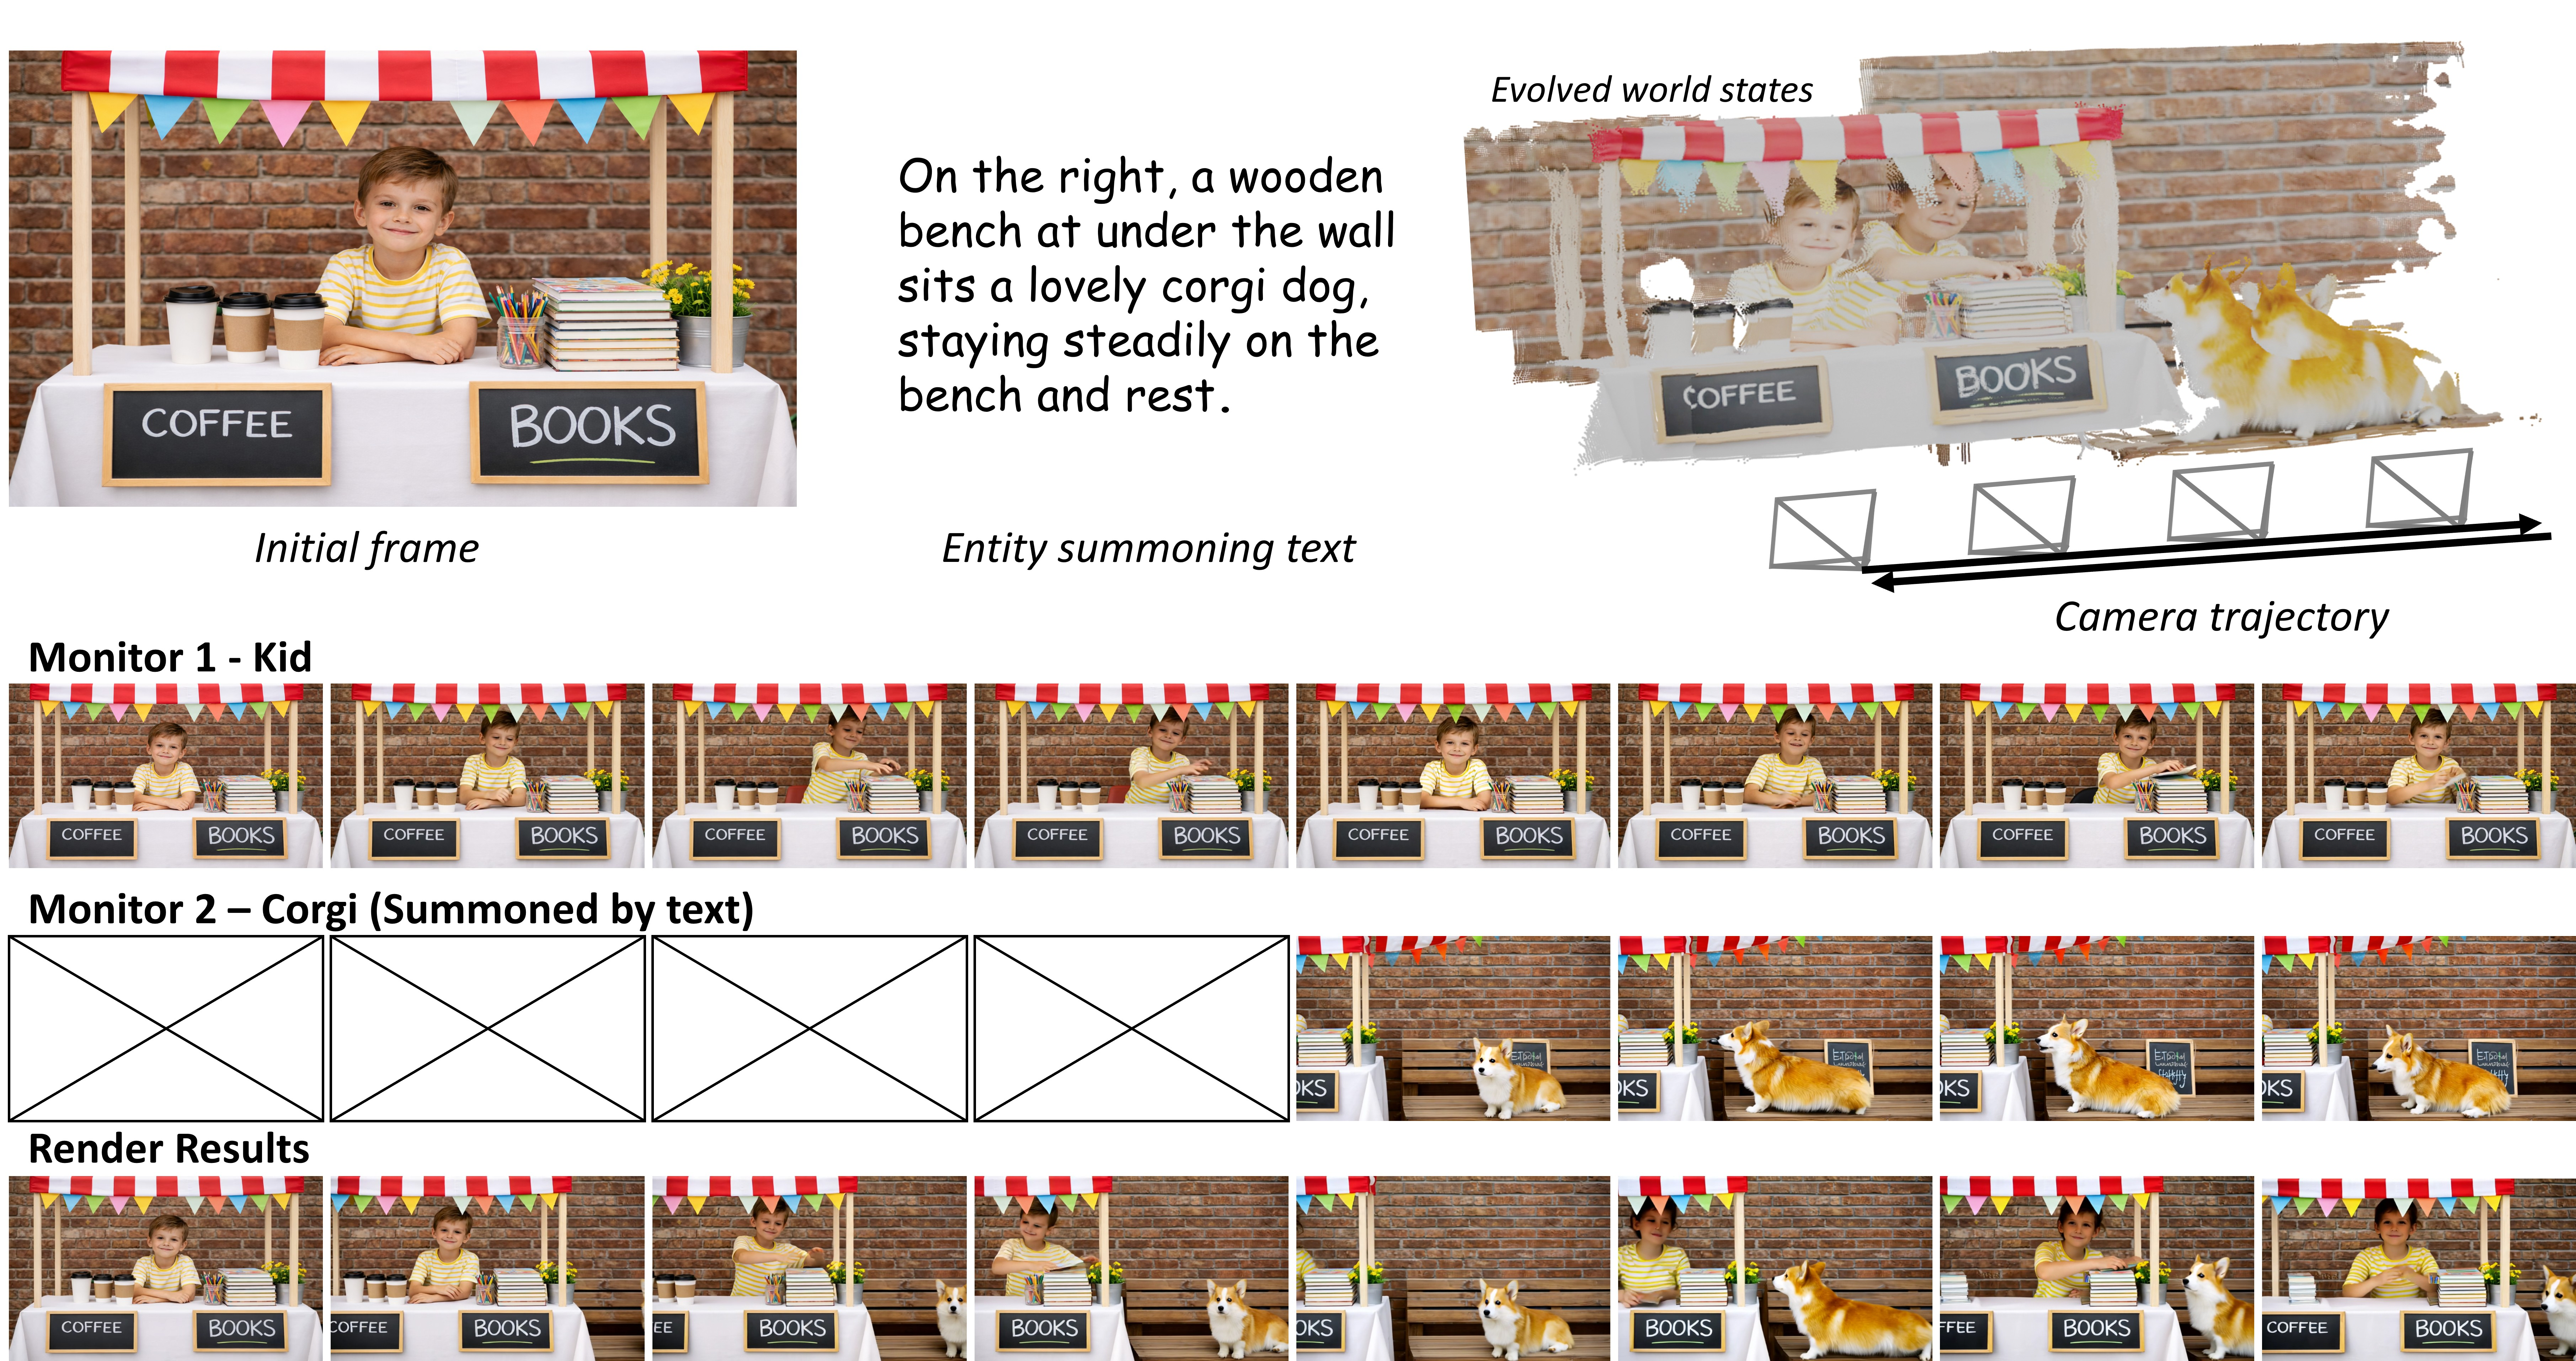
\includegraphics[width=1\linewidth]{imgs/multi.jpg}
    \caption{A demonstration of the late-appearing event revisiting. While we have the initial image containing the kid, we allow the renderer to generate the corgi following the text prompt. The monitor for the corgi is registered after the camera has overlap under the threshold with the monitor of the initial frame. The results showcase a perfect synchronization between the renderer and each monitor.}
    \label{fig:late_coming}
    % \vspace{-1mm}
\end{figure}

% --- 表 4：消融实验 ---
\begin{table}[t!]
\centering
\footnotesize
\setlength{\tabcolsep}{3pt}
\caption{Ablation studies of our proposed components. We validate the necessity of the evolution engine, spatial memory, and reference frames. The column in blue demonstrates the performance of a \textbf{\textcolor{cyan}{second revisit}}.}
\vspace{-1mm}
\label{tab:ablation}
\resizebox{\textwidth}{!}{
\begin{tabular}{l *{6}{c >{\columncolor{cyan!10}}c} | *{2}{c >{\columncolor{cyan!10}}c}}
\toprule
\multirow{3}{*}{\textbf{Method}} & \multicolumn{12}{c|}{\textbf{Same Pose Revisit}} & \multicolumn{4}{c}{\textbf{Different Pose Revisit}} \\
\cmidrule(lr){2-13} \cmidrule(lr){14-17}
& \multicolumn{2}{c}{$\text{PSNR}_{bg}\uparrow$} & \multicolumn{2}{c}{$\text{SSIM}_{bg}\uparrow$} & \multicolumn{2}{c}{$\text{LPIPS}_{bg}\downarrow$} & \multicolumn{2}{c}{$\text{CD}_{fg}\downarrow$} & \multicolumn{2}{c}{$\text{DINO}_{fg}\uparrow$} & \multicolumn{2}{c|}{\text{VQA-Acc}$\uparrow$} & \multicolumn{2}{c}{$\text{DINO}_{fg}\uparrow$} & \multicolumn{2}{c}{\text{VQA-Acc}$\uparrow$} \\
\cmidrule(lr){2-3} \cmidrule(lr){4-5} \cmidrule(lr){6-7} \cmidrule(lr){8-9} \cmidrule(lr){10-11} \cmidrule(lr){12-13} \cmidrule(lr){14-15} \cmidrule(lr){16-17}
& 1st & 2nd & 1st & 2nd & 1st & 2nd & 1st & 2nd & 1st & 2nd & 1st & 2nd & 1st & 2nd & 1st & 2nd \\
\midrule
w/o Event Evo.  & 20.005 & \textbf{18.995} & 0.671 & 0.647 & \textbf{0.299} & \textbf{0.315} & 4.215 & 5.431 & 0.425 & 0.401 & 18.512 & 13.985 & 0.380 & 0.350 & 18.105 & 12.855 \\
w/o Spa. Mem.   & 17.512 & 16.895 & 0.550 & 0.531 & 0.495 & 0.550 & 5.820 & 6.915 & 0.395 & 0.285 & 12.350 & 8.510  & 0.315 & 0.185 & 10.125 & 6.850 \\
w/o Ref. Frame  & 18.520 & 17.105 & 0.610 & 0.545 & 0.385 & 0.490 & 1.520 & 4.850 & 0.615 & 0.410 & 38.510 & 22.150 & 0.550 & 0.320 & 32.105 & 18.550 \\
\midrule
\textbf{Full} & \textbf{20.071} & 18.983 & \textbf{0.679} & \textbf{0.650} & 0.301 & 0.330 & \textbf{0.068} & \textbf{0.135} & \textbf{0.760} & \textbf{0.721} & \textbf{59.063} & \textbf{54.620} & \textbf{0.691} & \textbf{0.632} & \textbf{52.829} & \textbf{49.478} \\
\bottomrule
\end{tabular}
}
\vspace{-1mm}
\end{table}



% \vspace{-1mm}

% \section{Conclusion}
% We identify and formalize a fundamental limitation of existing generative video world models, the out-of-sight dynamics problem: unobserved regions are frozen at their last seen state, failing to capture ongoing events. To address this, we propose LiveWorld, a novel framework that explicitly decouples continuous world evolution from view-dependent rendering. By factorizing the environment into a temporally-invariant 3D background and explicitly evolving dynamic entities, LiveWorld makes global 4D evolution computationally tractable, overcoming the static-world assumption. Our monitor-centric pipeline uses virtual monitors to fast-forward unobserved entity dynamics and synchronize them with the global timeline, allowing the observer to maintain spatial coherence under explicit camera control in a persistently evolving world. We also introduce LiveBench, a benchmark for out-of-sight dynamics. Overall, LiveWorld establishes a principled foundation for long-term 4D world modeling, bridging the gap between static memorization and true dynamic simulation.

\vspace{-1mm}
\section{Conclusion}
We formalize the \textit{out-of-sight dynamics} problem in video world models, where unobserved regions incorrectly freeze at their last seen state. To overcome this, we propose LiveWorld, a framework that explicitly decouples continuous world evolution from view-dependent rendering. By factorizing the environment into a static 3D background and utilizing a monitor-centric pipeline to autonomously fast-forward unobserved active entities, LiveWorld achieves tractable 4D modeling. Along with LiveBench, our dedicated benchmark, LiveWorld bridges the gap between static 2D memorization and persistent 4D dynamic simulation.